\chapter{\selectlanguage{greek}Κώδικες Επανάληψης-Συσσώρευσης \en{(repeat - accumulate, RA)}}
\externaldocument{chapter1.tex}
\externaldocument{chapter2.tex}

Στο κεφάλαιο αυτό, παρουσιάζονται οι κώδικες Επανάληψης-Συσσώρευσης \en{(repeat - accumulate, RA)}, η μελέτη της επίδοσης των οποίων αποτελεί και το αντικείμενο της παρούσας εργασίας.

Οι \en{RA} αποτελούν τους πρώτους κώδικες που βασίζονται σε συσσωρευτές και εφευρέθηκαν από τους \en{D. Divsalar} κ .ά. \cite{divsalar1998coding}. Ενώ έχουν απλή δομή, δακρίνονται από καλές επιδόσεις, κυρίως στην κατεύθυνση της πρακτικής κωδικοποίησης \en{LDPC} κωδίκων των οποίων αποτελούν υποομάδα, με μοναδικό μειονέκτιμα ότι είναι γενικά χαμηλού ρυθμού (1/2 ή χαμηλότερου). Πλέον, χρηιμοποιούνται ήδη σε αρκετά πρότυπα τηλεπικοινωνιών (\en{DVB-S2,  WirelessMAN IEEE802.16}). Διακρίνονται ως μια ειδική κλαση των \textit{σειριακά συσσωρευμένων} κωδίκων (\en{serially concatenated codes - SC}), στους οποίους ο εξωτερικός κώδικας είναι ένας επαναληπτικός κώδικας ρυθμού $1/q$ και ο εσωτερικός είναι ένας συνελικτικός κώδικας γεννήτορα $\frac{1}{1+D}$, ο οποίος δίνει το $mod-2$ άθροισμα του \en{bit} εισόδου με το προηγούμενο \en{bit} εξόδου. Παράγει δηλαδή το άθροισμα όλων των παρελθόντων εισόδων και για το λόγο αυτό καλείται και \textit{συσσωρρευτής} (\en{accumulator}), στοιχείο που δίνει στος \en{RA} το όνομα τους.

\begin{figure}[h]
\center{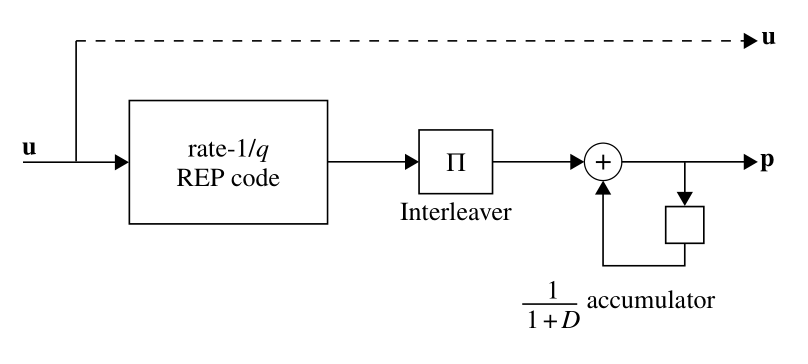
\includegraphics[width=0.65\linewidth]{figures/Ra_scheme.png}}
\caption{\en{Block} διάγραμμα ενός \en{RA} κώδικα}
\label{fig:RA scheme graph}
\end{figure}

Οι \en{RA} που μεταδίδουν τα \en{bits} πληροφορίας και τα \en{bits} ελέγχου ισοτιμίας λέγονται συστηματικοί. Ένα σχηματικό διάγραμα ενός συστηματικόυ \en{RA} κώδικα, φαίνεται στο Σχήμα \ref{fig:RA scheme graph}. Η αποκωδικοποίησή τους μπορεί να αντιμετωπισθεί είτε ως σειριακή \en{turbo}, είτε ως \en{LDPC}, τακτική που είναι και πιο η ευρέως διαδεδομένη \cite{ryan2009channel}.


Στη συνέχεια του κεφαλαίου παρουσιάζονται συνοπτικά οι κώδικες που μπορούν να πλησιάσουν το θεωρητικό όριο χωρητικότητας που επιβάλει το θεώρημα \en{Shannon} (Θεώρημα \ref{theorem:shannon}), διατηρώντας παράλληλα τη δυνατότητα πρακτικής κωδικοποίησης και αποκωδικοποίησης. Αφού γίνει μια σύντομη αναφορά στη σχέση χωρητικότητας και σηματοθορυβικής σχέσης (\en{SNR}), παρουσιάζονται οι τρόποι διαχείρησης των \en{RA}, είτε ως \en{turbo}, είτε ως \en{LDPC}. Κατόπιν αφού αναλυθεί ο τρόπος κωδικοποίησης των \en{LDPC} (ως τον πιο συχνά χρησιμοποιούμενο τρόπο αντιμετώπισης των \en{RA}), διατυπώνεται πλήρως το \en{coding scheme} των \en{RA}, που δίνει και τη βάση πάνω στην οποία στηρίζεται η προσομοίωση που έγινε και θα αναλυθεί στο Κεφάλαιο 4.

\section{Κώδικες που πλησιάζουν τη χωρητικότητα}

Μέχρι και πολύ πρόσφατα, οι κώδικες που μπορούσαν να λειτουργήσουν κοντά στο θεωρητικό όριο χωρητικότητας που προέβλεπε το θεώρημα \en{Shannon}, ήταν κυρίως μεγάλοι σε μήκος, μη πρακτικοί κώδικες. Με την ανακάλυψη των \en{turbo} κωδίκων και την επανανακάλυψη των \en{LDPC} τη δεκαετία του '90, έγινε δυνατό να αποδειχθεί η ικανότητα λειτουργίας τους κοντά στη χωρητικότητα, με πρακτικά υλοποιήσιμους κωδικοποιητές-αποκωδικοποιητές σε σχετικά μεσαία \en{bit error rates (BERs)}, μέσω του καναλιού \en{AWGN}. 

Παρ'όλο που η θεωρητική επίτευξη του ορίου χωρητικότητας αφορά κώδικες με άπειρο μήκος, στην πράξη αρκεί το μήκος του κώδικα να είναι αρκετά μεγάλο (π.χ. $n\geq5000$) ώστε να υπάρχει ικανοποιητική απόδοση κοντά στο θεωριτικό όριο. Η σχεδίαση τέτοιων κωδίκων χαρακτηρίζεται από 2 βασικά στοιχεία:
\begin{itemize}
\item Χρήση κωδίκων αποτελούμενων από απλά μέρη, συνενωμένα με τρόπο που να παράγεται μια ψευδο-τυχαία κατανομή βαρών και,
\item Χρήση μη-βέλτιστων επαναληπτικών αλγορίθμων αποκωδικοποίησης με συνεχή ανταλλαγή \en{soft} πληροφορίας, των οποίων η πολυπλοκότητα αυξάνει γραμμικά με την αύξηση του μήκους κώδικα.
\end{itemize}

Μπορεί επίσης να δοθεί και ο παρακάτω ορισμός των κωδίκων που πλησιάζουν τη χωρητικότητα:
\begin{definition}\en{Capacity-approaching} κώδικες

Έστω μια αλληλουχία από δυαδικούς γραμμικούς κώδικες $\left( C_m \right)$, ρυθμού $R_m$ και για κάθε κώδικα, οι κωδικές λέξεις μεταδίδονται ισοπίθανα μέσω ενός καναλιού με χωρητικότητα $C$. Η αλληλουχία επιτυγχάνει κλάσμα $1-\epsilon$ της χωρητικότητας του καναλιού αν $\lim_{m\to \infty}R_m\geq\left(1-\epsilon\right)\cdot C$ και υπάρχει αλγόριθμος αποκωδικοποίησης για τον οποίο η πιθανότητα εσφαλμένου \en{bit} του κώδικα $C_m$ τείνει στο μηδέν, όταν $m\to \infty$ \cite{pfister2005capacity}.
\label{def:capacity approaching codes}
\end{definition}

Οι \en{capacity-approaching} κώδικες χωρίζονται σε δύο μεγάλες υποκατηγορίες: τους \en{turbo} ή \en{turbo-like} κώδικες, οι οποίοι διακρίνονται από συνελικτικούς \en{component codes} χαμηλής πολύπλοκότητας και κάνουν χρήση του επαναληπτικού αποκωδικοποιητή αθροίσματος γινομένου (\en{sum-product decoder}) και τους κώδικες Πίνακα Ισοτιμίας Χαμηλής Πυκνότητας (\en{Low Density Parity Check - LDPC}).

\begin{figure}[h]
\center{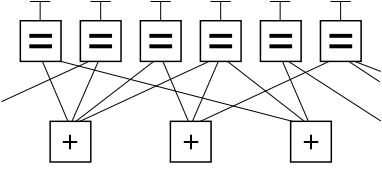
\includegraphics[width=0.65\linewidth]{figures/LDPC_factor_graph.png}}
\caption{Μέρος του γραφήματος παραγόντων ενός \en{LDPC} κώδικα}
\label{fig:LDPC factor graph}
\end{figure}


Οι \en{LDPC} κώδικες, κατά κύριο λόγο χρησιμοποιούν \en{component codes} μονού ελέγχου ισοτιμίας και επαναληπτική ανταλλαγή μυνημάτων (με τη μορφή πιθανοτήτων) για την αποκωδικοποίηση, που βασίζεται σε διμερή γραφήματα. Και οι δύο κατηγορίες που περιγράφηκαν, διακρίνονται από κοινά στοιχεία. Kάνοντας χρήση γενικής αναπαράστασης με γραφήματα παραγόντων (\en{factor-graph representation}) οι \en{turbo} κώδικες θεωρούνται πλέον μια γενίκευση των \en{LDPC}. Επίσης πλέον, όλοι οι \en{capacity-approaching} κώδικες μπορούν να ομαδοποιηθούν ως οικογένεια Κωδίκων σε Γραφήματα (\en{Codes on Graphs}) \cite{ryan2009channel}, \cite{johnson2009iterative}, \cite{codes2009guest}.

\subsection{Η χωρητικότητα ως \en{SNR}}

Σε αυτό το σημείο θα γίνει μια σύντομη αναφορά στη σχέση που συνδέει τη χωρητικότητα ενός καναλιού με τη σηματοθορυβική σχέση \en{SNR} που το χαρακτηρίζει.

Έστω τηλεπικοινωνιακό σύστημα, με ζωνοπερατό κανάλι, εύρους ζώνης $W$, που εισάγει \en{AWGN} θόρυβο, με φασματική πυκνότητα ισχύος $N_0/2$. Η χωρητικότητα καναλιού αποδεικνύεται ότι μπορεί να οριστεί από την παρακάτω εξίσωση (Θεώρημα \en{Shannon - Hartley}):

\begin{equation}
C=W\cdot log_2(1+ \frac{S}{N})
\label{eq:capacity}
\end{equation}
όπου, $S$ η λαμβανόμενη ισχύς του μεταδιδόμενου σήματος στο δέκτη, $N$ η ισχύς θορύβου και $W$ το εύρος ζώνης του καναλιού. Από την εξίσωση \ref{eq:capacity} καθώς και το Σχήμα \ref{fig:Channel capacity}, διακρίνονται οι δύο οριακές περιπτώσεις για την τιμή της χωρητικότητας σε σχέση με το \en{SNR}.
\begin{itemize}
\item Για μεγάλα \en{SNR} ($SNR \gg 0$) η χωρητικότητα εκφράζεται από τη σχέση $C\approx W\log_{2}{\frac{S}{N}}$, είναι δηλαδή λογαριθμικής δύναμης και σχεδόν γραμμική σε σχέση με το εύρος ζώνης. Η περιοχή αυτή καλείται \textit{\en{bandwidth-limited regime}}
\item Για μικρά \en{SNR} ($SNR \ll 0$) η χωρητικότητα εκφράζεται από τη σχέση $C\approx W\cdot\frac{S}{N}\log_{2}{e}$, είναι δηλαδή γραμμικής δύναμης αλλά δεν επηρεάζεται από το εύρος ζώνης. Η περιοχή αυτή καλείται \textit{\en{power-limited regime}}
\end{itemize}


\begin{figure}[h]
\center{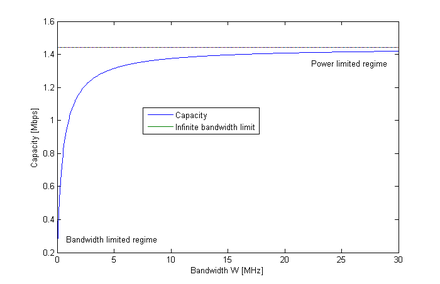
\includegraphics[width=0.55\linewidth]{figures/Channel_capacity.png}}
\caption{Χωρητικότητα ζωνοπερατού καναλιού ως προς το εύρος ζώνης}
\label{fig:Channel capacity}
\end{figure}

Η ισχύς του θορύβου δίνεται από τη σχέση:

\begin{equation}
N = \int_{-W}^{W}\frac{N_0}{2}\,df=N_0\cdot{W}.
\label{eq:Noise}
\end{equation}
,ενώ η συματοθορυβική σχέση του συστήματος (\en{signal-to-noise ratio - SNR}) ορίζεται ως:

\begin{equation}
SNR=\frac{S}{N}
\label{eq:SNR}
\end{equation}

Από τις \ref{eq:capacity} και \ref{eq:SNR} και κανονικοποιώντας ως προς το εύρος ζώνης $W$, προκύπτει:

\begin{equation}
C=log_2(1+SNR)
\label{eq:capacity vs SNR}
\end{equation}
σχέση που αποτελεί και το άνω όριο του ρυθμού για αξιόπιστη επικοινωνία σύμφωνα με το Θεώρημα \ref{theorem:shannon} (Θεώρημα Κωδικοποίησης Ενθόρυβου Καναλιού).

\section{\en{RA} ως \en{turbo}}

Σε αυτή την παράγραφο, θα γίνει μια σύντομη αναφορά στους κώδικες \en{turbo}, της ιδιότητες που χαρακτηρίζουν την αποκωδικοποίησή τους, καθώς και την δυνατότητα των \en{RA} να χαρακτηριστούν ως τέτοιοι.

\subsection{Κώδικες \en{turbo}}

Οι κώδικες \en{turbo} ανακαλύφθηκαν από τους \en{Berrou, Glavieux} και \en{Thitimajshima} \cite{berrou1993near} το 1993 και αποτέλεσαν ριζοσπαστική προσέγγιση της κωδικοποίησης για διόρθωση σφαλμάτων. Αποτελούνται από τον παράλληλο συνδυασμό δύο συνελικτικών κωδίκων, οι οποίοι κατά την αποκωδικοποίηση διαμοιράζουν πληροφορία μεταξύ των αντίστοιχων αποκωδικοποιητών. Αναφέρεται πως ο κωδικοποιητής χρησιμοποιεί συνελικτικούς κώδικες \cite{hagenauer1996iterative}, ενώ ο αποκωδικοποιητής χρησιμοποιεί \en{BCJR} κώδικες \cite{abrantes2004bcjr}.

\begin{figure}[h]
    \centering
    \begin{minipage}{0.45\textwidth}
        \centering
        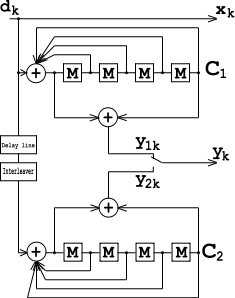
\includegraphics[width=0.9\textwidth]{figures/Turbo_encoder.png}
        \caption{Κωδικοποιητής \en{turbo}}
    \end{minipage}\hfill
    \begin{minipage}{0.45\textwidth}
        \centering
        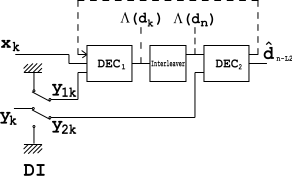
\includegraphics[width=0.9\textwidth]{figures/Turbo_decoder.png}
        \caption{Αποκωδικοποιητής \en{turbo}}
    \end{minipage}
\end{figure}

Ο κωδικοποιητής \en{turbo} περιέχει έναν \textit{παρεμβολέα} (\en{interleaver}), ο ρόλος του οποίου είναι να μεταθέτει κωδικές λέξεις μικρού βάρους από τον ένα κωδικοποιητή σε κωδικές λέξεις μεγάλου βάρους στον άλλο, με διάφορους τρόπους. Επιγραμματικά αναφέρεται ο \en{\textit{row-column} interleaver}, o \en{\textit{helical}} kai o \en{\textit{odd-even} interleaver}.

Η αποκωδικοποίηση απαιτέι τον υπολογισμό πιθανοτικών μετρικών \en{log-likelihood ratios (LLRs)} και την πρόβλεψη για το μεταδιδόμενο σύμβολο $\mathbf{y_k}$, με βάση την εγγύτητά του στο 0 ή στο 1, καθώς και χρησιμοποιώντας \en{Hard-Desicion} αποκωδικοποίηση \cite{berrou1993near}.

\subsection{\en{RA} ως \en{turbo}}

Το συνολικό \en{coding scheme} των \en{RA} που προσομοιώθηκε θα αναλυθεί στη συνέχεια του κεφαλαίου. Ωστόσο, η αποκωδικοποίηση τους μπορεί να βασιστεί στην \en{turbo} αποκωδικοποίηση των \en{SC}, όπου, όπως αναφέρθηκε ήδη, ο εξωτερικός κώδικας είναι \en{repetition} και ο εσωτερικός είναι ο \en{accumulator}. Για τους συστηματικούς \en{RA} κώδικες που περιέχουν συνδυαστή, ο εσωτερικός κώδικας είναι συνδυαστικός αποκωδικοποιητής συνδυαστή-συσσωρευτή (\en{accumulator-combiner - AC}) και ο \en{REP} αποκωδικοποιητής έχει ως είσοδο τα \en{LLRs} από το κανάλι \cite{johnson2009iterative}.

\begin{figure}[h]
\center{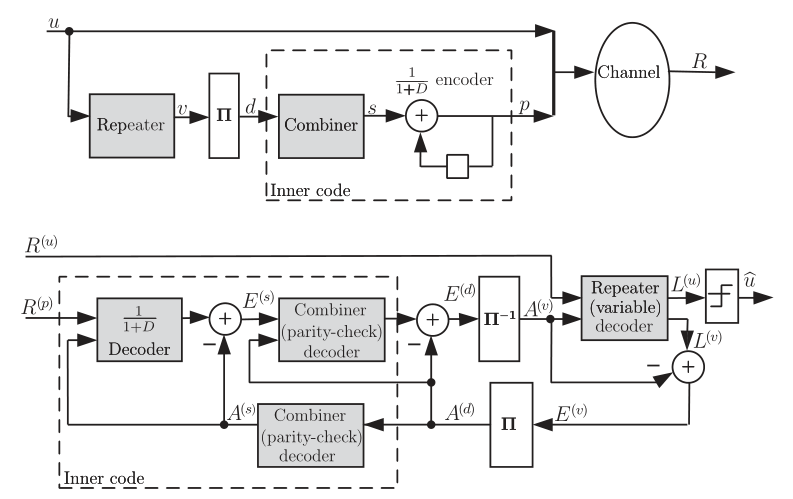
\includegraphics[width=0.85\linewidth]{figures/systematic_RA.png}}
\caption{Κωδικοποιητής / \en{turbo} αποκωδικοποιητής συστηματικού \en{RA}}
\label{fig:enc/turbo dec of systematic RA}
\end{figure}

Στο Σχήμα \ref{fig:enc/turbo dec of systematic RA}, φαίνεται η κωδικοποίηση και αποκωδικοποίηση \en{turbo} ενός \en{RA} κώδικα, βάση της \textit{αρχής \en{turbo}} (\en{turbo principle}) \cite{hagenauer2003turbo}. Σε κάθε επανάληψη της αποκωδικοποίησης, ο \en{REP} αποκωδικοποιητής λαμβάνει \en{LLRs} από το κανάλι αναφορικά με τα \en{bits} πληροφορίας και στις επόμενες επαναλήψεις, τα \en{a-priori LLRs} εξωγενούς πληροφορίας από τον \en{AC} αποκωδικοποιητή, από τις προηγούμενες επαναλήψεις.

Στο επόμενο βήμα ο \en{REP} αποκωδικοποιητής υπολογίζει τα \en{LLRs} εξόδου. Η εξωγενής πληροφορία από τον \en{REP} αποκωδικοποιητή, παρεμβάλλεται από τον \en{interleaver} για την παραγωγή \en{a-priori LLRs} στον \en{AC} αποκωδικοποιητή. Στην τελική επανάληψη, υπολογίζεται η κωδική λέξη από τα \en{a posteriori LLRs} για τα \en{bits} πληροφορίας από το κανάλι και τα \en{a-priori LLRs} από τον \en{AC} αποκωδικοποιητή για τα κωδικά \en{bits}. Ο αλγόριθμος τελειώνει μετά από ένα προκαθορισμένο αριθμό $I_{max}$ επαναλήψεων. Σε περίπτωση μη-συστηματικού \en{RA} τα υπολογιζόμενα \en{LLRs} για τα \en{bits} πληροφορίας είναι μηδέν \cite{johnson2009iterative}.


\section{\en{RA} ως \en{LDPC}}

Οι κώδικες \en{LDPC} παρουσιάστηκαν για πρώτη φορά το 1962 από τον \en{R. G. Gallager} στη διδακτορική του διατριβή \cite{gallager1962low} και αποτελούν κώδικες διόρθωσης σφαλμάτων που ορίζονται από αραιό πίνακα ελέγχου ισοτιμίας. Παρά το ότι αποτελούν \en{capacity-approaching} κώδικες εγκαταλείφθηκαν για περίπου 30 χρόνια, με εξαίρεση τη δουλειά του \en{Tanner} \cite{tanner1981recursive} που εισήγε και τη γραφική αναπαράσταση τους, μέσω του γραφήματος \en{Tanner}, λόγω περιορισμών στην τεχνική τους υλοποίηση και επανακαλύφθηκαν το 1996 από τους \en{Mackay} κ.α. \cite{mackay1996near}. Tο κύριο χαρακτηριστικό τους, η χαμηλή πυκνότητα του πίνακα $\mathbf{H}$, είναι και αυτό που κάνει τους \en{LDPC} να επιδέχονται διάφορους αλγόριθμους επαναληπτικής αποκωδικοποίησης (\en{iterative decoding}). Παρ’ότι οι αλγόριθμοι επαναληπτικής αποκωδικοποίησης έχουν μη-βέλτιστη απόδοση, μπορούν να έχουν απόδοση που χαρακτηρίζεται “σχεδόν” βέλτιστη (\en{near-optimal}), σε εφαρμογές/\en{error-rates} ενδιαφέροντος και διακρίνονται από καλύτερες επιδόσεις στη διόρθωση σφαλμάτων σχετικά με τους \en{turbo}.

Κάθε γραμμικός κώδικας έχει αναπαράσταση μέσω πίνακα ελέγχου-ισοτιμίας, ωστόσο για να αποτελεί \enquote*{αραιή} η αναπαράσταση πρέπει να πλοιρούνται ορισμένα κριτήρια. Ένας $n\times m$ πίνακας καλείται αραιός αν το ποσό από άσσους (1) στις γραμμές και στις στήλες του, το βάρος γραμμών ($w_r$) και στηλών ($w_c$) αντίστοιχα, είναι πολύ μικρότερο από τις διαστάσεις του ($w_r\ll m$, $w_c\ll n$). Πρακτικά, θεωρείται πως αν το $1\%$ των στοιχείων του πίνακα είναι άσσοι, τότε εί77ναι αραιός. Αν το βάρος γραμμών και στηλών είναι σταθερό ο κώδικας \en{LDPC} λέγεται ομαλός, ενώ σε αντίθετη περίπτωση λέγεται ανώμαλος \cite{ta2013tutorial}.

Γενικά, εκτός από την απαίτηση να είναι ο πίνακας $\mathbf{H}$ αραιός, οι \en{LDPC} δε διαφέρουν από τους \en{block} κώδικες. Ωστόσο, η εύρεση ενός αραιού πίνακα ελέγχου ισοτιμίας για ένα δεδομένο \en{block} κώδικα αποτελεί δύσκολη διαδικασία και αντίθετα της κατασκευής των \en{LDPC} προηγείται η κατασκευή του πίνακα $\mathbf{H}$ και ακολουθεί η σχεδίαση του κωδικοποιητή. Λόγω αυτού οι \en{LDPC} αποκωδικοποιούνται επαναληπτικά, κάνοντας χρήση γραφικής αναπαράστασης του πίνακα ελέγχου ισοτιμίας και σχεδιάζονται με γνώμονα τις ιδιότητές του.

Έχει διαπιστωθεί πως και οι \en{RA} και οι  \en{LDPC} ενέχουν πλεονέκτημα σε σχέση με τους \en{turbo} κώδικες, καθώς προσφέρουν μια πιο ευέλικτη δομή, κάτι που με τη σειρά του προσφέρει περισσότερους βαθμους ελευθερίας στην επιλογή των παραμέτρων για δεδομένο κριτήριο σχεδίασης \cite{johnson2009iterative}.

\subsection{Κωδικοποίηση \en{LDPC}}

Όπως αναφέρθηκε στο Κεφάλαιο 2, οι γραμμικοί \en{block} κώδικες αποτυπώνουν το μήνυμα πληροφορίας $\mathbf{u}$ στην κωδική λέξη $\mathbf{v}$ κάνοντας χρήση της εξίσωσης \ref{eq:check equation}, για δοσμένο γεννήτορα πίνακα $\mathbf{G}$. Γενικά, όπως έχει επίσης αναφερθεί και στο Κεφάλαιο 2, ο πίνακας $\mathbf{G}$ ενός κώδικα δίνεται από το \en{null-space} του -αραιού για τους \en{LDPC}- πίνακα $\mathbf{H}$. Συνεπώς είναι απίθανο να είναι και ο ίδιος αραιός, κάτι που θα οδηγούσε σε γραμμικό χρόνο κωδικοποίησης (ως προς το μήκος του κώδικα). Προκύπτει επομένως πως, η κωδικοποίηση ενός \en{LDPC} με βάση την εξίσωση \ref{eq:check equation} γίνεται σε τετραγωνικό χρόνο ως προς το μήκος κώδικα. Σημειώνεται πως έχουν γίνει διάφορες προσπάθειες προς την κατεύθυνση της μείωσης του χρόνου αυτού \cite{ta2013tutorial}. Ωστόσο, οι κώδικες \en{LDPC} κατασκευάζονται με γνώμονα τον πίνακα ελέγχου ισοτιμίας $\mathbf{H}$. Συνεπώς, η κωδικοποίησή τους, ακολουθεί διαφορετική πορεία. 

Αρχικά, το μήνυμα πληροφορίας αποτυπώνεται στην κωδική λέξη ως εξής:

\begin{equation}
\begin{split}
\mathbf{v} &= \mathbf{G}^T\mathbf{u} \\
\Rightarrow \mathbf{0} &= \mathbf{H}\mathbf{G}^T\mathbf{u} \\
\Rightarrow \mathbf{0} &= \mathbf{H}\mathbf{G}^T
\end{split}
\label{eq:LDPC encoding}
\end{equation}

Θεωρώντας συστηματική κωδικοποίηση, και υπενθυμίζοντας πως ο συστηματικός γεννήτορας πίνακας μπορεί να γραφεί ως $\mathbf{G} = \left[\mathbf{P}\;\;\mathbf{I_k}\right]$, προκύπτει πως

\begin{equation}
\begin{split}
\mathbf{H}\mathbf{G}^T &= \mathbf{H_1}\mathbf{I_k} + \mathbf{H_2}\mathbf{P}^T \\
\Rightarrow \mathbf{P}^T &= \mathbf{H_2}^{-1}\mathbf{H_1}
\end{split}
\label{eq:parity part of LDPC}
\end{equation}
και λαμβάνοντας υπ'όψη την εξίσωση \ref{eq:LDPC encoding} προκύπτει η κωδική λέξη (σχηματικά στο Σχήμα \ref{fig:LDPC codeword formation})

\begin{equation}
\mathbf{v} = \mathbf{G}^T\mathbf{u} = \left[\mathbf{P}\;\;\mathbf{I_k}\right]^T\mathbf{u} = \left[\mathbf{u}\;\;\mathbf{H_2}^{-1}\mathbf{H_1}\mathbf{u}\right]^T
\label{eq:LDPC codeword formation}
\end{equation}

\begin{figure}[h]
\center{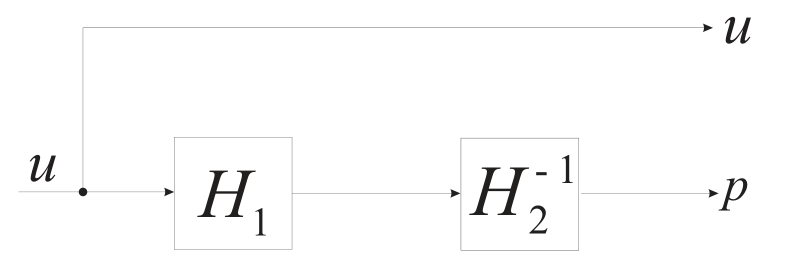
\includegraphics[width=0.75\linewidth]{figures/LDPC_encoding.png}}
\caption{Διαμόρφωση συστηματικής κωδικής λέξης \en{LDPC} κώδικα}
\label{fig:LDPC codeword formation}
\end{figure}

\subsection{Κωδικοποίηση \en{RA}}

Το \en{block} διάγραμμα διαμόρφωσης της κωδικής λέξης ενός \en{RA} κώδικα, δόθηκε ήδη στο Σχήμα \ref{fig:RA scheme graph}. Η κωδικοποίηση \en{RA} ακολουθεί την συστηματική \en{LDPC}. Τα \en{bits} πληροφορίας αντιγράφονται $q$ φορές, περνούν από τον παρεμβολέα, ομαδοποιούνται μέσω $mod-2$ πρόσθεσης σε \en{block} μήκους $a$ και τέλος περνούν από ένα συνελικτικό κωδικοποιητή μνήμης -1.

Συγκεκριμένα, το μήνυμα πληροφορίας μήκους $k$, $\mathbf{u}=\left(u_0,u_1,\cdots,u_{k-1}\right)$, μετά την έξοδο από τον επαναληπτικό κωδικοποιητή, έχει τη μορφή:

\begin{equation}
\begin{split}
\mathbf{c} &= \left[c_1, c_2, \cdots, c_{qk} \right] \\
&= (\underbrace{u_1,u_1,\cdots,u_1}_q, \; \underbrace{u_2,u_2,\cdots,u_2,}_q, \; \cdots, \; \underbrace{u_{qk},u_{qk},\cdots,u_{qk}}_q)
\end{split}
\end{equation}
, όπου $c_i=u_{f(i)}$ με $f(i)=\lceil i/q \rceil$ και $\lceil x \rceil$ το άνω κατώφλι του $x$.

Κατόπιν, κατα την έξοδο από τον παρεμβολέα $\Pi=[\pi_1,\pi_2,\cdots,\pi_{qk}]$, διαμορφώνεται μια μετάθεση της ακολουθίας $\mathbf{c}$ ως εξής:

\begin{equation*}
\mathbf{d} = \left[d_1, d_2, \cdots, d_{qk} \right] = [c_{\pi_1}, c_{\pi_2}, \cdots, c_{\pi_{qk}}]
\end{equation*}

Ο συνδυαστής λαμβάνει την έξοδο του παρεμβολέα και προσθέτει ($mod-2$) και ομαδοποιεί τα \en{bits} σε \en{block} μήκους $a$. Τα \en{bits} της ακολουθίας εξόδου του συνδυαστη $\mathbf{s}$, δίνονται από την εξίσωση:

\begin{equation}
s_i=d_{a(i-1)+1}\oplus d_{a(i-1)+2} \oplus \cdots \oplus d_{ai}, \;\;\; i=1,2,\cdots,m\;\;m=kq/a
\label{eq:combiner equation}
\end{equation}

Στην έξοδο του συσσωρευτή, τα \en{parity bits} θα δίνονται από την εξίσωση:

\begin{equation}
p_i=p_{i-1}\oplus s_i\;\;\; i=1,2,\cdots,m
\label{eq:accumulator equation}
\end{equation}

Από την εξίσωση \ref{eq:accumulator equation}, προκύπτει πως η κωδική λέξη του συστηματικού \en{RA} κώδικα, έχει τη μορφή $\mathbf{v}=[u_1, u_2,\cdots,u_k,p_1,p_2,\cdots,p_m]$, οπότε το μήκος του κώδικα προκύπτει $n=k(1+q/a)$ και ο ρυθμός $R=a/(a+q)$ \cite{johnson2009iterative}.

\subsection{Αποκωδικοποίηση \en{RA}}

Αναφέρθηκε ήδη η δυνατότητα των \en{RA} κωδίκων για \en{turbo} αποκωδικοποίηση. Ωστόσο, στο πλαίσιο της συγκεκριμένης εργασίας, μελετάται η δυνατότητα για αποκωδικοποίηση ως \en{LDPC}, χρησιμοποιώντας τον αλγόριθμο \en{\textit{Sum-Product}}.

Ο αλγόριθμος παρουσιάστηκε από τον \en{Gallager} μαζί με τους κώδικες \en{LDPC}. Χαρακτηρίζεται από \en{near-optimal} επίδοση αποκωδικοποίησης καθώς και από καθολικότητα για τα διάφορα κανάλια χωρίς μνήμη (\en{BEC, BSC, BI-AWGN}, κ.λ.π.), συνεπώς η ανάπτυξή του είναι γενική. Το κριτήριο βέλτιστης ανάπτυξης του αλγορίθμου, είναι ο υπολογισμός της μέγιστης εκ των υστέρων (\en{maximum a posteriori - MAP}) πιθανότητα. Υπολογίζεται δηλαδή η (εκ των υστέρων) πιθανότητα για την τιμή κάθε συγκεκριμένου \en{bit} της κωδικής λέξης $\mathbf{v}$, με δεδομένο το ληφθέν διάνυσμα $\mathbf{r}$.

\subsubsection{Ο \en{Sum-Product} αλγόριθμος για \en{LDPC}}

Η αποκωδικοποίηση του κωδικού \en{bit} $v_j$ (χωρίς βλάβη της γενικότητας) απαιτεί τον υπολογισμό της \en{APP} πιθανότητας (για τιμή \en{bit} 1):
\begin{equation*}
\Pr(v_j=1|\mathbf{r})
\end{equation*}
το λόγο \en{APP}
\begin{equation*}
l(v_j|\mathbf{r})\triangleq\frac{\Pr(v_j=0|\mathbf{r})}{\Pr(v_j=1|\mathbf{r})}
\end{equation*}
ή το (σταθερότερο αριθμητικά) λόγο \en{log-APP}, που καλείται επίσης \en{log-likelihood ration (LLR)}:

\begin{equation}
L(v_j|\mathbf{r})\triangleq\log\left(\frac{\Pr(v_j=0|\mathbf{r})}{\Pr(v_j=1|\mathbf{r})}\right)
\label{eq:LLR}
\end{equation}

\begin{figure}[h]
\center{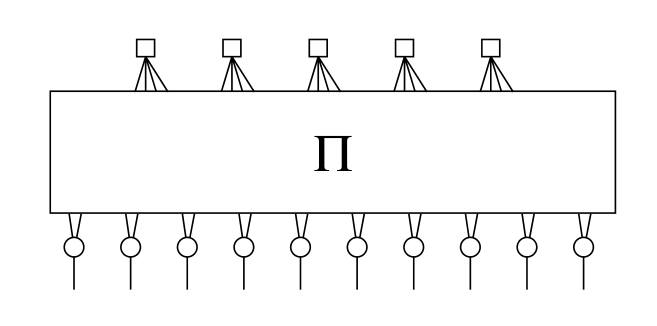
\includegraphics[width=0.6\linewidth]{figures/LDPC_graphical.png}}
\caption{Αναπαράσταση \en{LDPC} ως αλληλουχία από \en{SPC} (κάτω) και \en{REP} (επάνω) κώδικες. Με $\Pi$ συμβολίζεται ο παρεμβολέας}
\label{fig:LDPC graphical}
\end{figure}

Ο υπολογισμός της εξίσωσης \ref{eq:LLR} γίνεται εφαρμόζοντας την αρχή \en{turbo} στο γράφημα \en{Tanner}. Με αναφορά το Σχήμα \ref{fig:LDPC graphical}, ο \en{LDPC} μπορεί να θεωρηθεί ως ένα σύνολο από \en{SPC} κώδικες συνδεόμενους μέσω του παρεμβολέα σε ένα σύνολο \en{REP} κωδίκων. Οι \en{SPC} κώδικες (\en{CNs} στο γράφημα \en{Tanner}) θεωρούνται εξωτερικοί κώδικες, συνεπώς δε συνδέονται στο κανάλι.

Τα Σχήματα \ref{fig:VN}, \ref{fig:CN} αναπαριστούν στιγμιότυπα των \en{REP} και \en{SPC} αποκωδικοποιητών (κόμβοι \en{VN} και \en{CN} αντίστοιχα).

\begin{figure}[h]
    \centering
    \begin{minipage}{0.45\textwidth}
        \centering
        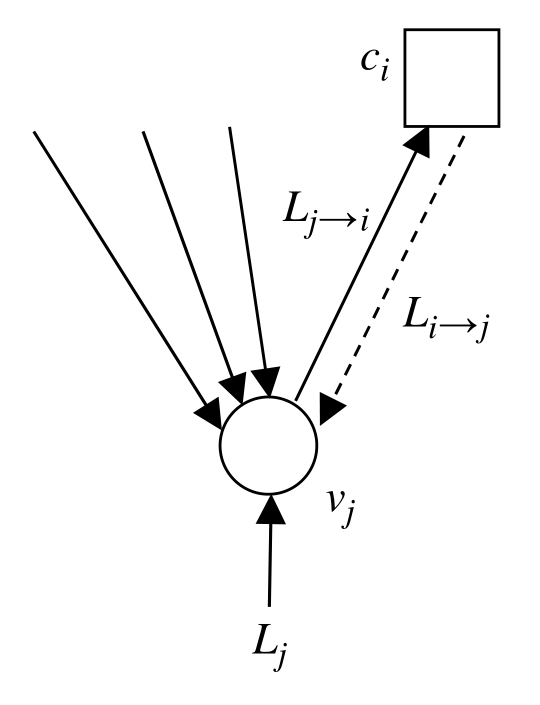
\includegraphics[width=0.9\textwidth]{figures/VN.png}
        \caption{Ο κόμβος \en{VN} $j$ (αποκωδικοποιητής κώδικα \en{REP}) λαμβάνει πληροφορία από τους γειτονικούς \en{CN} (εκτός από τον $i$ $(L_{i\to j})$) και στέλνει στον \en{CN} $i$ την ποσότητα $L_{j\to i}$}
        \label{fig:VN}
    \end{minipage}\hfill
    \begin{minipage}{0.45\textwidth}
        \centering
        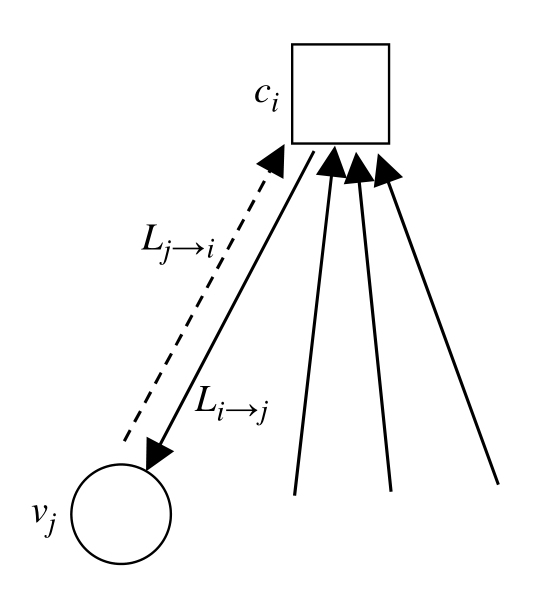
\includegraphics[width=0.9\textwidth]{figures/CN.png}
        \caption{Ο κόμβος \en{CN} $i$ (αποκωδικοποιητής κώδικα \en{SPC}) λαμβάνει πληροφορία από τους γειτονικούς \en{VN} (εκτός από τον $j$ $(L_{j\to i})$) και στέλνει στον \en{VN} $j$ την ποσότητα $L_{i\to j}$}
        \label{fig:CN}
    \end{minipage}
\end{figure}

Οι αποκωδικοποιητές (κόμβοι) \en{VN} και \en{CN} λειτουργούν συνεργατικά για τον υπολογισμό της εκτίμησης $L(v_j|\mathbf{r}),\;\;j=0,1,\cdots,n-1$, επαναληπτικά. Κατά τη λειτουργία τους, υιοθετείται το \en{\textit{flooding schedule}}, σύμφωνα με το οποίο ξεκινώντας από τους \en{VN}, οι \en{VN} (\en{CN}) επεξεργάζονται την είσοδο και υπολογίζουν \textit{εξωγενή πληροφορία} την οποία στέλνουν στους γειτονικούς \en{CN} (\en{VN}). Η διαδικασία ολοκληρώνεται μετά από ένα προκαθορισμένο αριθμό επαναλήψεων ή αφού εκπληρωθεί ένα κριτήριο τερματισμού και υπολογίζεται η πιθανότητα $L(v_j|\mathbf{r})$, μέσω της οποίας λαμβάνεται απόφαση για την τιμή του \en{bit} $v_j$. Η υλοποίηση του \en{SPA} βασίζεται επίσης στη \textit{υπόθεση ανεξαρτησίας}: οι ληφθείσες ποσότητες \en{LLR} σε κάθε κόμβο από τους γειτονικούς, είναι μεταξύ τους ανεξάρτητες.

Θα χρειαστεί να αναφερθούν επίσης οι εσωτερικές διαδικασίες και υπολογισμοί, που λαμβάνουν χώρα στους κόμβους \en{VN} και \en{CN} αντίστοιχα, για τον υπολογισμό της μετρικής \en{LLR} που ανταλλάσσεται μεταξύ γειτονικών κόμβων. Θεωρείται πως αντί για \en{MAP} αποκωδικοποιητές, οι \en{VN} και \en{CN} λειτουργούν σαν \en{APP} επεξεργαστές για \en{REP} και \en{SPC} κώδικες αντίστοιχα, σε κάθε επανάληψη του αλγορίθμου.

Η εξωγενής πληροφορία που στέλνεται από τον \en{VN} $j$ στον \en{CN} $i$ δίνεται από τη εξίσωση:

\begin{equation}
L_{j\to i} = L_j + \sum_{i'\in N(j)-\lbrace i\rbrace} L_{i'\to j}
\label{eq:CN update}
\end{equation}
, όπου η ποσότητα $L_j$ δίνεται από την εξίσωση \ref{eq:LLR}. Αντίστοιχα, η εξωγενής πληροφορία που στέλνεται από τον \en{CN} $i$ στον \en{VN} $j$, δίνεται από την παρακάτω εξίσωση:

\begin{equation}
L_{i\to j} = 2\tanh^{-1} \left( \prod_{j'\in N(i)-\lbrace j\rbrace} \tanh \left( \frac{1}{2}L_{j'\to i} \right)\right)
\label{eq:VN update}
\end{equation}
Στο τέλος των επαναλήψεων, ο \en{VN} $j$ παράγει μια πρόβλεψη με βάση την ποσότητα

\begin{equation}
L_{j}^{total} = L_j + \sum_{i\in N(j)} L_{i\to j}
\label{eq:LLR total}
\end{equation}

Η πληροφορία $L_{j\to i}$ που ανταλάσσεται μεταξύ των \en{VN} $j$ και \en{CN} $i$, απότελεί τη βέλτιστη (εξωγενή) εκτίμηση της τιμής του $v_j$ (πρόσημο του $L_{j\to i}$) και το επίπεδο εμπιστοσύνης της τιμής (πλάτος του $L_{j\to i}$), βασισμένη στο \en{REP constraint} για τον αντίστοιχο κόμβο. Αντίστοιχα, η εκτίμηση του \en{CN} $i$ βασίζεται στο \en{SPC constraint}. Τέλος αναφέρεται πως για την αρχικοποίηση, χρησιμοποιείται η εξίσωση \ref{eq:LLR}, η οποία διαμορφώνεται διαφορετικά για κάθε τύπο διακριτού καναλιού χωρίς μνήμη. Ενδεικτικά, για το δυαδικό \en{AWGN} κανάλι, προκύπρει η σχέση:

\begin{equation}
L(v_j|r_j) = \frac{2r_j}{\sigma^2}
\label{eq:AWGN initial LLR}
\end{equation}

Τέλος, ο αλγόριθμος απαιτεί ένα κριτήριο τερματισμού. Χρησιμοποιείται η εξίσωση
\begin{equation*}
\mathbf{v}\mathbf{H}^T=\mathbf{0}
\end{equation*}
, όπου $\mathbf{v}$ είναι μια δοκιμαστικά υπολογισμένη εκτίμηση της κωδικής λέξης \cite{ryan2009channel}, \cite{johnson2009iterative}, \cite{ta2013tutorial}.

\subsubsection{Ο \en{Sum-Product} αλγόριθμος για \en{RA}}

Αναφέρθηκε ήδη πως οι εξισώσεις \ref{eq:combiner equation} και \ref{eq:accumulator equation}, είναι οι εξισώσεις ελέγχου ισοτιμίας για ένα \en{RA} κώδικα. Η κωδικοποίηση είναι συστηματική, συνεπώς οι πρώτες $k$ στήλες του πίνακα $\mathbf{H}$ αντιστοιχούν στα \en{bits} πληροφορίας, ενώ οι επόμενες $m=n-k$ στήλες στα \en{parity bits}. Αναφέρθηκε επίσης πως ο πίνακας $m\times n \mathbf{H}$ είναι της μορφής

\begin{equation}
H=[H_1\;H_2]
\label{eq:RA parity check matrix form}
\end{equation}
όπου ο υποπίνακας $H_1$ είναι πίνακας $n-k\times k$ με βάρη γραμμών και στηλών, $(a,q)$ αντίστοιχα και ο $H_2$ οφείλεται στον \en{accumulator}.

Παρόμοια με τους \en{LDPC} κώδικες, το γράφημα \en{Tanner} των \en{RA} κωδίκων ορίζεται από τον πίνακα $\mathbf{H}$, με διαφορά ότι είναι εμφανής η διάκριση μεταξύ \en{info bits} και \en{parity bits}. Στο Σχήμα \ref{fig:RA tanner graph} φαίνεται το γράφημα \en{Tanner} ενός \en{RA}, στο οποίο γίνεται διάκριση μεταξύ των $k$ συστηματικών \en{bits} βαθμού $q$ στην κορυφή και των $m$ \en{parity bits} κόμβων βαθμού 2 (πλην του τελευταίου που διακρίνεται από βαθμό 1). Οι κόμβοι ελέγχου του γραφήματος διακρίνονται από βαθμό $a+2$, εκτός του τελευταίου που έχει βαθμό $a+1$ \cite{johnson2009iterative}.

\begin{figure}[H]
\center{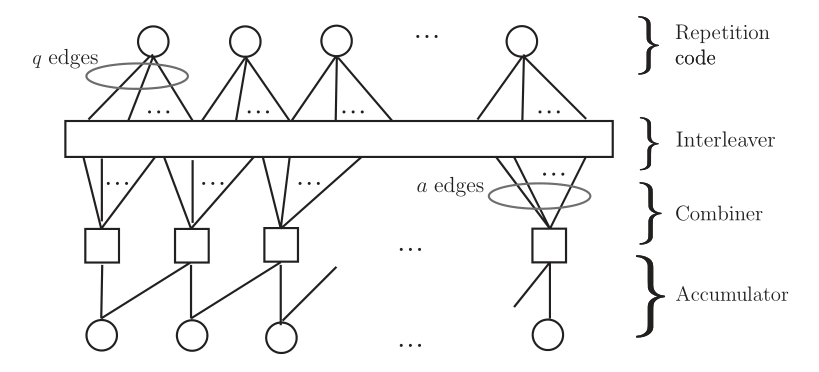
\includegraphics[width=0.85\linewidth]{figures/Ra_tanner.png}}
\caption{Γράφημα \en{Tanner RA} κώδικα}
\label{fig:RA tanner graph}
\end{figure}

Στην περίπτωση που οι κόμβοι \en{parity bits} και συστηματικών \en{bits} αντιμετωπίζονται ως ενιαίοι κόμβοι \en{bits} ο αλγόριθμος \en{SPA} για \en{RA} κώδικα, ταυτίζεται με αυτόν για ένα \en{LDPC} που έχει τον ίδιο πίνακα $\mathbf{H}$. Σε αντίθετη περίπτωση απαιτούνται τροποποιήσεις για τη συμπλήρωση μιας επανάληψης του αλγορίθμου.

Τέλος, ως σύγκριση μεταξύ του \en{Sum-Product} αποκωδικοποιητή και της \en{turbo} αποκωδικοποίησης, αναφέρεται πως, ενώ στον \en{SPA} οι \en{parity bit} κόμβοι αποκωδικοποιούνται όμοια με τους \en{systematic bit} κόμβους, ο \en{turbo} αποκωδικοποιητής χρησιμοποιεί \en{BCJR} αποκωδικοποιητή με διάγραμμα \en{trellis}. Μέσω αυτού οι επαναλήψεις της \en{turbo} αποκωδικοποίησης είναι πιο πολύπλοκες, ωστόσο απαιτούνται λιγότερες επαναλήψεις συνολικά \cite{ryan2009channel}, \cite{johnson2009iterative}.